% !TEX root = mythesis.tex

%==============================================================================
\chapter{Source follow-up analysis}
\label{chap:follow-up}
%==============================================================================

One of the most exciting fields of modern day neutrino astrophysics involves scanning the observable sky to look for neutrino sources. As mentioned in section~\ref{subsubsec:Nusources} the observation of TXS 0506+056~\cite{Icecube_txs} and NGC 1068~\cite{Icecube_2022} which are examples of a transient source and a steady state of neutrinos has brought unprecedented excitement to the field. Any observation of a neutrino source offers a chance to significantly increase our overall knowledge about astroparticle physics. Since, Auger is one of the few experiments in the world sensitive to UHE$\nu_s$ (E > $10^{16}$eV) any improvement in its point source sensitivity increases its capability for neutrino detection. 

In this chapter, the point source sensitivity to $\nu$ events of the SD array is discussed for the zenith angular range explored in this thesis, DG$_{\text{low}}$. Based on the zero neutrino candidates found in the search performed in this work a source declination, $\delta$ dependent neutrino flux is calculated. This process includes calculating the declination dependent exposure and then converting it to a limit on the flux. The improvements to this exposure and sensitivity by the inclusion of new triggers is also discussed. Finally, the new limit is used to scan a few interesting sources which lie in the most sensitive range for the DG$_{\text{low}}$ region.

\section{Procedure for point source analysis}
\label{sec:procedure_point_source}

\subsection{Source visibility}
\label{subsec:psource_coverage}
The field of view (FOV) of the Observatory and the corresponding neutrino efficiency is related to the zenith angle which in turn is related to the declination. For a given point-like source at declination $\delta$ and right ascension $\alpha$ (in equatorial coordinates), the time zenith angle which is the $\theta$ dependence at a certain time, $t$ is given by:
\begin{equation}
  \label{eq:zenith_angle_time}
  cos \theta(\text{t}) = sin \lambda \,sin \delta+ cos \lambda \, cos \delta \,sin (2\pi \frac{\text{t}}{\text{T}} - \alpha)
\end{equation} 
where $T$ is the duration of one sidereal day and $\lambda$ is the latitude of the observer ($\lambda = -35.2^{\circ}$ for Pierre Auger Observatory). 
Fig.~\ref{fig:Auger_FoV} shows the FOV bands for different neutrino search channels (DG$\mathrm{_{\text{low}}}$, DG$\mathrm{_{\text{high}}}$, ES). These bands are plotted in equatorial coordinates as a function of $\mathrm{\alpha - t _{GS}}$ where $\mathrm{t_{GS}}$ is the Greenwich Sidereal Time (GST) converted to for a mean longitude of the Observatory, $l$ calculated as $\mathrm{t_{GS}= 2\pi t/T + l}$. The sensitive declination ranges for different $\mathrm{t_{GS}}$ can be read from the plot which is very useful for real-time transient follow-up. For DG$\mathrm{_{\text{low}}}$ showers the SD of the Pierre Auger Observatory is sensitive to declinations between $\delta \sim -85^{\circ} - 40^{\circ}$. Another way to denote sky coverage for different neutrino searches at Auger is by calculating the time a source is visible to the Observatory for a particular declination. This is plotted in fig.~\ref{fig:time_per_day} for all three search channels. As it can be seen from the plot all three channels are the most sensitive at two ends of their sensitive declination ranges (DG$\mathrm{_{\text{low}}}$-$\delta \sim -70^{\circ}, 35^{\circ}$) which is a consequence of smaller variation in zenith angle in time for certain directions. The sensitivity sharply decreases beyond these declination values. In the middle of these \textit{two horns} is a plateau like region. It is also seen that generally the fraction of time a source is visible is comparable in the DG$\mathrm{_{\text{low}}}$ and DG$\mathrm{_{\text{high}}}$ channel with both being higher than the ES channel due to the size of the zenith angle windows. The fraction of visible time for vertical showers is also plotted. Even though this fraction of time is significantly high, currently no neutrino search is performed for this region as it is very difficult to differentiate between a cosmic ray and neutrino EAS for this zenith angle range.

\begin{figure}[t!]
  \centering
  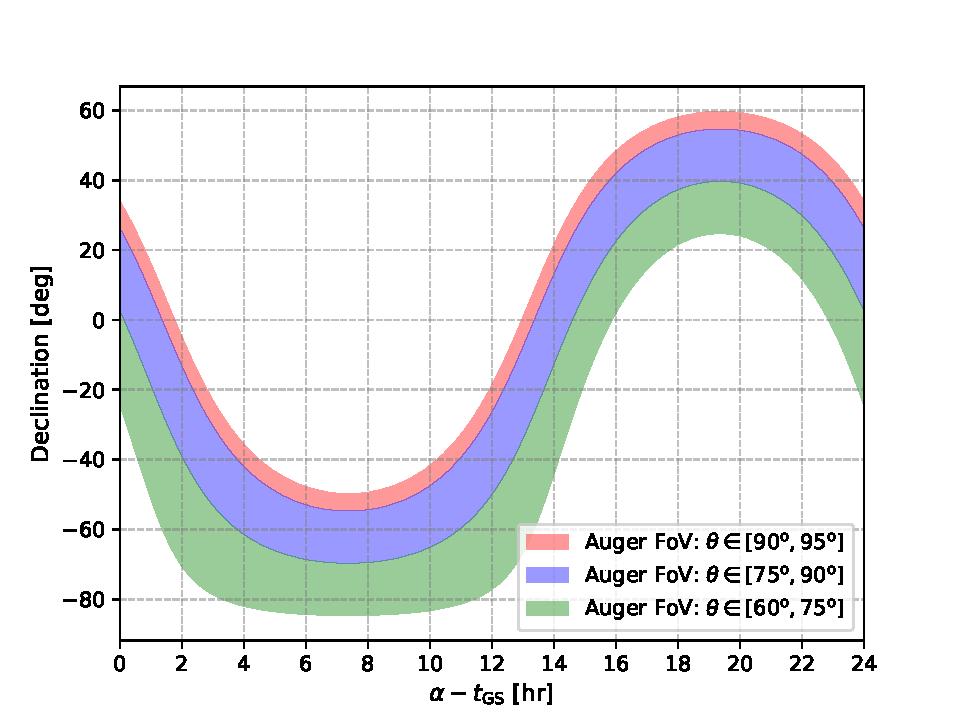
\includegraphics[width=14.5cm]{thesis_figures/PointLimits/Auger_FoV_1.pdf}
  \caption{Instantaneous field of view for different neutrino searches performed at the Pierre Auger Observatory. The declination is plotted as a function of $\alpha - t_{GS}$ where $t_{GS}$ is the Greenwich Sidereal Time converted to the mean longitude of the Observatory. The bands show the sensitive declination ranges for different neutrino searches (ES: red, DGH: blue, DGL: green) which are separated based on zenith angle ranges.}
  \label{fig:Auger_FoV}
\end{figure}

\begin{figure}[t!]
  \centering
  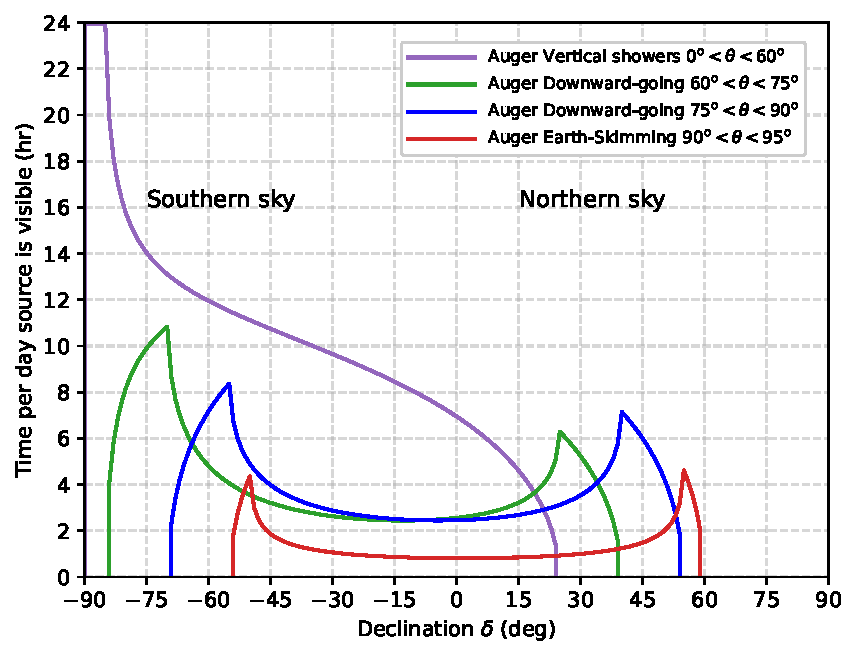
\includegraphics[width=14.5cm]{thesis_figures/PointLimits/Time_per_day.pdf}
  \caption{Total time per sidereal day a source is visible to the Pierre Auger Observatory for different neutrino searches. The time is plotted as a function of declination. The ES channel is shown in red while the DG$\mathrm{_{\text{low}}}$ and DG$\mathrm{_{\text{high}}}$ channels are shown in green and blue respectively. The fraction of time a source is visible for vertical showers is also shown in purple.}
  \label{fig:time_per_day}
\end{figure}

\subsection{Effective area and Exposure}
\label{subsec:psource_area}
Following this to calculate point source sensitivity, the declination dependent SD exposure is evaluated. This is done by first calculating an effective area to neutrinos of flavours i and energy $E_{\nu}$ is defined in the following way. For a point source spectral flux of flavour $i$ given by $\phi_i(E_{\nu}) = \frac{d^4 N_{\nu}}{dE_{\nu} dA dt}$ the expected number of detected events is given by 

\begin{equation}
  \label{eq:expected_events_point}
  \frac{dN_{i}}{dt} = \int_{E_{\nu_{\text{min}}}}^{E_{\nu_{\text{max}}}} \, dE_{\nu} \, \phi(E_{\nu}) \, \mathcal{A}_i(E_{\nu})
\end{equation}
The effective area is flavour dependent since for each flavour the shower development and the primary interaction (c = NC, CC) is substantially different. The effective area is for the DG$\mathrm{_{\text{low}}}$ region is given as follows:
\begin{equation}
  \label{eq:effective_area}
  \mathcal{A_{i,c}}(E_{\nu},\theta(t),t) = \frac{\sigma^{i,c}(E_{\nu})}{m_N} \int_{X} \, \varepsilon_{i,c}(E_{\nu},\theta(t),t) \, A_{6T5} n_{\text{hex}}(t) \, dX
\end{equation}

\begin{figure}[t!]
  \centering
  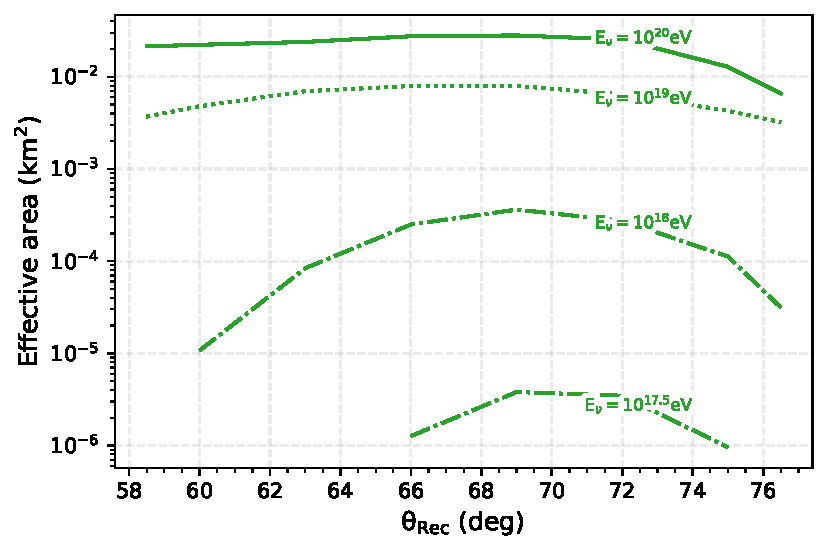
\includegraphics[width=14.5cm]{thesis_figures/PointLimits/EffArea_vs_Theta_CC_optim.pdf}
  \caption{Instantaneous effective area for $\nu_e$ CC neutrinos as a function of zenith angle for different neutrino energies. The effective area is calculated for the DG$\mathrm{_{\text{low}}}$ channel.}
  \label{fig:Eff_Area}
\end{figure}


, where $\varepsilon_{i,c}$ is the neutrino identification efficiency for a 6T5 unit. The declination dependence is taken into account by the $\theta(t)$ dependence of the efficiency. The instantaneous effective area for electron neutrinos with CC interactions in km$^2$ and different theta is plotted in fig.~\ref{fig:Eff_Area}. The effective area increases with increasing primary energy. It also increases with zenith angles till $\sim$70$^\circ$ after which there is a slight decrease in the effective area which is due to the decrease in neutrino sensitivity at higher zenith angles discussed earlier in section~\ref{subsec:nu_sel_nudeteff}. 

The exposure to point-like sources of UHE neutrinos can then be calculated by integrating the effective area for a given time interval and summing over the different flavours (1:1:1 expectation at Earth ) and channels as follows:
\begin{equation}
  \label{eq:exposure_point}
  \xi(E_{\nu}, \delta) = \sum_{i,c} \int_{t} \mathcal{A_{i,c}} \, (E_{\nu},\theta(t),t) \, dt
\end{equation}


\begin{figure}[t!]
  \centering
  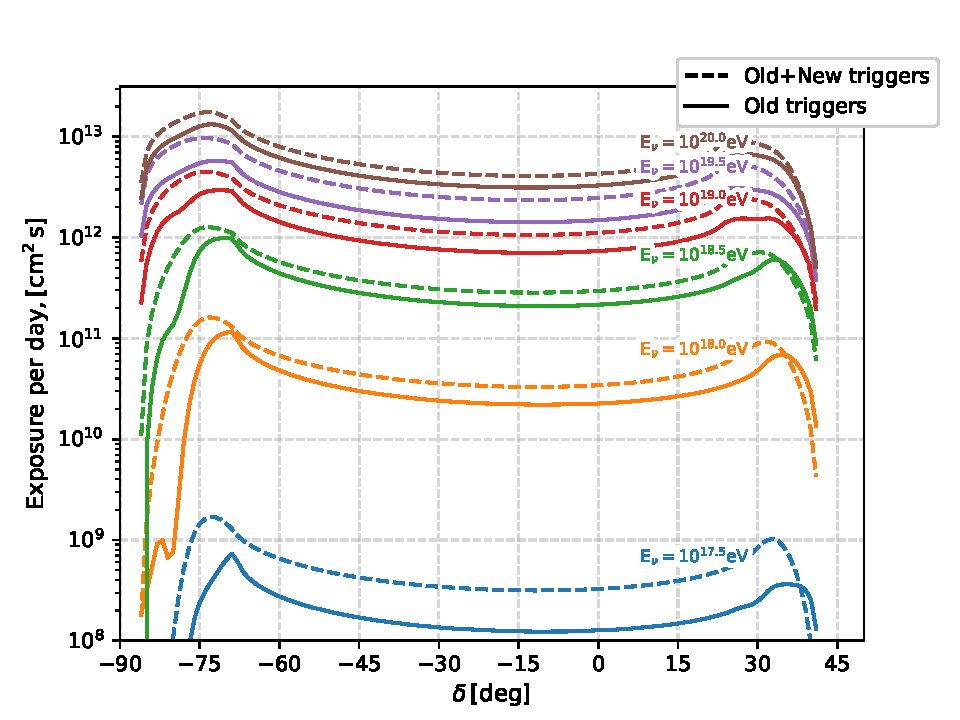
\includegraphics[width=14.5cm]{thesis_figures/PointLimits/Exposure_vs_Dec.pdf}
  \caption{Average exposure for different neutrino energies as a function of declination for the DG$\mathrm{_{\text{low}}}$ channel. The exposure is calculated for the time period 2014-2021. The solid lines show the exposure calculated with the previous analysis while the dashed lines show the exposure calculated with the inclusion of new triggers.}
  \label{fig:Exp_dec}
\end{figure}

\begin{figure}[t!]
  \centering
  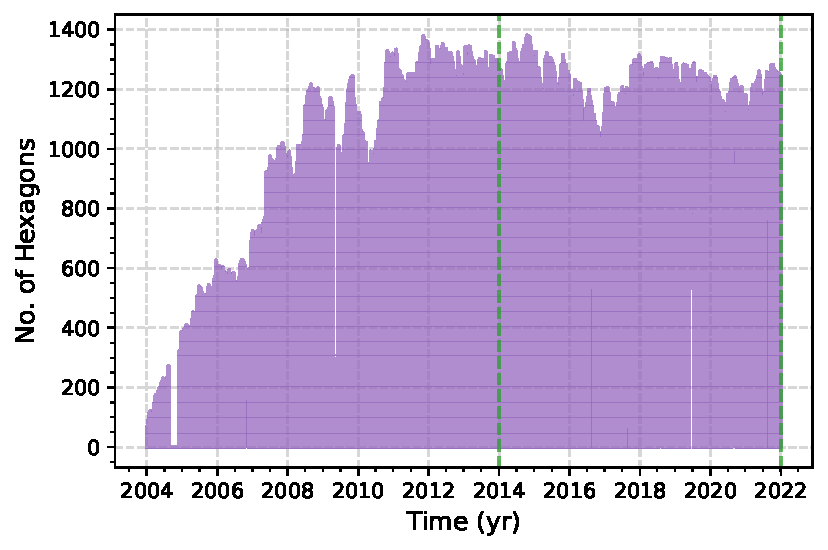
\includegraphics[width=14.5cm]{thesis_figures/PointLimits/Hexagons_2004_2021_forSrijan.pdf}
  \caption{Number of 6T5 hexagons as a function of time. The white regions show the outages which are removed from the searches. The area between the green lines shows the time period of this search.}
  \label{fig:Hexagon_time}
\end{figure}

The exposure is $\delta$ dependent due to the dependence of effective area on $\theta(t)$. The effective area can also change with time due to the changes in the number of hexagons $n_{hex}(t)$. This change has been visualized in fig.~\ref{fig:Hexagon_time}. As it can be seen in the plot the number is relatively stable especially in the period of one sidereal day apart from a few outages which are removed from the searches. The directional exposure for the DGL channels for different fixed energies between 2014-2021 is shown in fig.~\ref{fig:Exp_dec}. The dashed line shows the exposure calculated in this study by including the new triggers while the solid line shows the exposure calculated with the previous analysis for the same time period. Similar to the exposure calculated for the diffuse flux the exposure is significantly improved for lower energies with the improvement decreasing for higher energies. The shape of the exposure is similar to the observation time plot in fig.~\ref{fig:time_per_day} with the maximum exposure peaks seen at the same declinations. 

% As it can be seen in~\cite{} ES exposure published in~\cite{} is also plotted for comparison. It can be seen that generally the DG$_{low}$ point source exposure is lower than that of ES expect at higher energies where it is comparable. At these energies the different sensitive zenith angle ranges between the channels are the only differentiating factors for the exposure distribution. 

\section{Point-source neutrino flux limit}
\label{sec:pfux_limit}
Since no neutrino candidate was discovered in the search window an upper limit to a  point-like source of UHE neutrinos can be calculated. Similar to the calculation for the diffuse flux the number of expected neutrino events from a point like source at a given declination can be written as:

\begin{equation}
  N_{\text[expected]}(\delta) = \int_{E_{\text{min}}}^{E_{\text{max}}}  \phi(E_{\nu}) \, \xi(E_{\nu}, \delta) \, dE_{\nu}
\end{equation}

The point source flux is assumed to be independent of time and is assumed to be characterized as a power law, $\phi(E_{\nu}) = k_{\text{PS}} E_{\nu}^{-2}$ for all declinations. The integrated upper-limit from each source can then be further calculated as follows:

\begin{equation}
  \label{eq:point_flux_limit}
  k_{\text{PS}}^{90\%CL} = \frac{N_{\text{Up}}}{\int_{E_{\text{min}}}^{E_{\text{max}}} E_{\nu}^{-2} \, \xi(E_{\nu}, \delta) \, dE_{\nu}}
\end{equation}

For this study initially a time period from 1 Jan 2014 till 31 December 2021 is selected. The N$_{\tetx{Up}}$ = 2.39 is calculated according to the Conrad approach as mentioned in section~\ref{subsec:Conrad}. The exposure is assumed to be uniform within $\pm 0.6\%$ for the time period of search as shown in~\cite{PierreAuger:2017pzq}. 


\begin{figure}[t!]
  \centering
  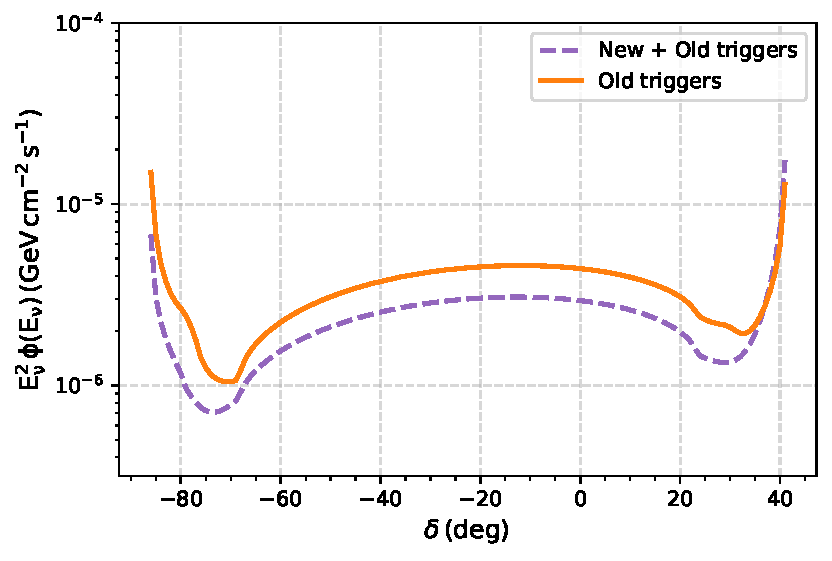
\includegraphics[width=14.5cm]{thesis_figures/PointLimits/Point_comp_new_old.pdf}
  \caption{Comparison of the 90\% C.L. declination dependent upper-limit (01.01.2004 - 31.12.2021) for the DG$_{\text{low}}$ channel of a single flavor point-like flux of UHE . The limit (dashed line) is compared to the limit obtained from the previous analysis (solid line) for the same time period.}
  \label{fig:Dec_limit_new old}
\end{figure}

The 90\% C.L. declination dependent upper-limit for the DG$_{\text{low}}$ channel is shown in fig.~\ref{fig:Dec_limit_new old}. The limit is the stringent for the times the source is seen the longest. The limit is calculated for the energy range $\sim$ 2.0 $\times 10^{18}$eV - $\times 10^{20}$eV. The dependence of energy intervals is minimal. This limit is also compared to the limit obtained from the previous analysis for the same time period in the same figure. As it can be seen the limit is significantly improved with new triggers fulfilling one of the primary objectives of this thesis. Further a combined limit is calculated where the old analysis is applied for the time period 01.01.2004 - 31.12.2013 and the analysis presented in this thesis is applied for the time period 01.01.2014 - 31.12.2021. This combination is only done under the assumption that the systeamtics for both the time periods are similar and 0 neutrino candidates were found in both time periods. This combination along with the limits from the separate time periods is shown in Fig.~\ref{fig:Dec_limit_comb1}. Further this combination is also compared to the point-like source limit calculated with the old analysis for the time period 01.01.2004-31.12.2021. This is presented in fig.~\ref{fig:Dec_limit_comb2}. For the best declination range of the DG$_{\text{low}}$ channel the limit is improved by a factor of $\sim$ 2.5???.
\todo{Get this number }

\begin{figure}[t!]
  \centering
  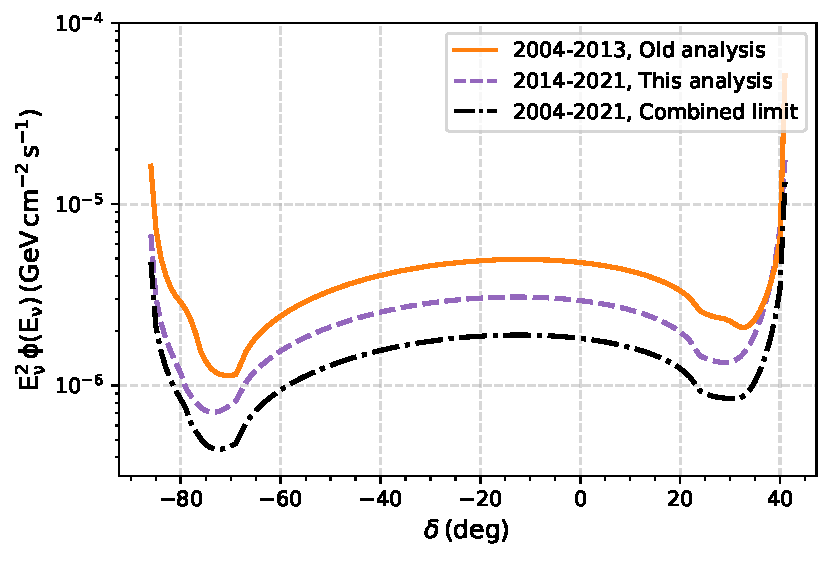
\includegraphics[width=14.5cm]{thesis_figures/PointLimits/Point_comp_combined.pdf}
  \caption{Limit comparison}
  \label{fig:Dec_limit_comb1}
\end{figure}

\begin{figure}[t!]
  \centering
  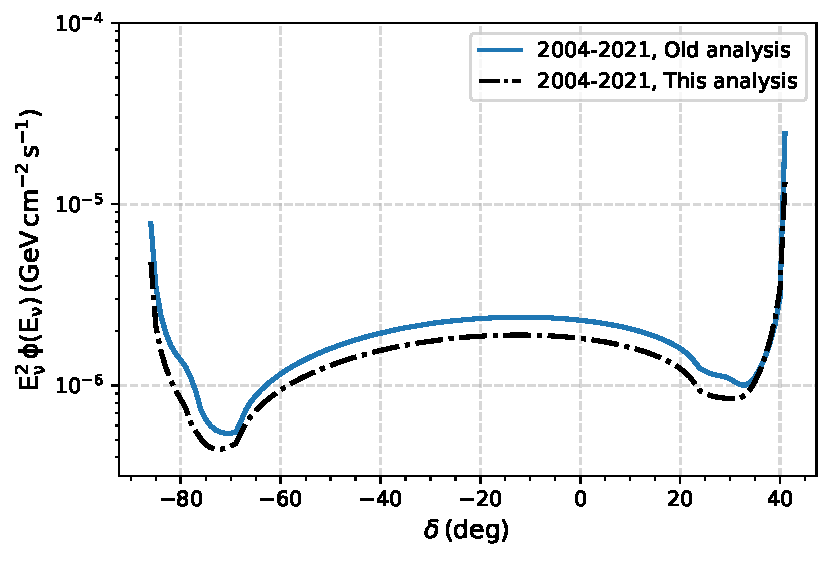
\includegraphics[width=14.5cm]{thesis_figures/PointLimits/Point_comp_combined_2.pdf}
  \caption{Limit comparison 2}
  \label{fig:Dec_limit_comb2}
\end{figure}

A cross-check of the diffuse limit is obtained from the point source analysis by performing double integration of the exposure, $\xi(E_{\nu}, \delta)$ in a similar way as done in~\cite{gap_note_2013}.

The diffuse limit can be written as:
\begin{equation}
  \mathrm{k_{PS}^{90\%CL} < \frac{N_{Up}}{\int_{log_{10}E_{min}}^{log_{10}E_{max}} \int_{-\pi/2}^{\pi/2}2\pi \cdot cos(\delta) \cdot E_{\nu}^{-1} \cdot \xi(E_{\nu}, \delta) \cdot ln(10) \cdot d(log_{10}(E_{\nu})) \cdot d\delta}} 
\end{equation}

\todo{Calculate this }
The diffuse limit from point source analysis is given as: 
\begin{equation}
  \mathrm{k_{PS}^{90\%CL} < 2.0000 \times 10^{-8} GeV cm^{-2} s^{-1} sr^{-1}}
\end{equation}

\todo{Write a bit more about crosschecks}
Which agrees with the value mentioned in eq.~\ref{eq:final_lim}. It is also important to mention that even though the overall sensitive declination range for the DG$_{\text{low}}$ analysis is small in comparison to other channels~\cite{Aab_2019_point}, the improvement presented in this thesis is still important as the sensitive declination ranges are not fully overlapping. Thus, if there is a point source at between declinations $ \delta \in [-80^{\circ}- -68^{\circ}]$ then DG$_{\text{low}}$ channel offers the only window at Auger to see UHE$\nu_s$ from such a source.  

\begin{figure}[t!]
  \centering
  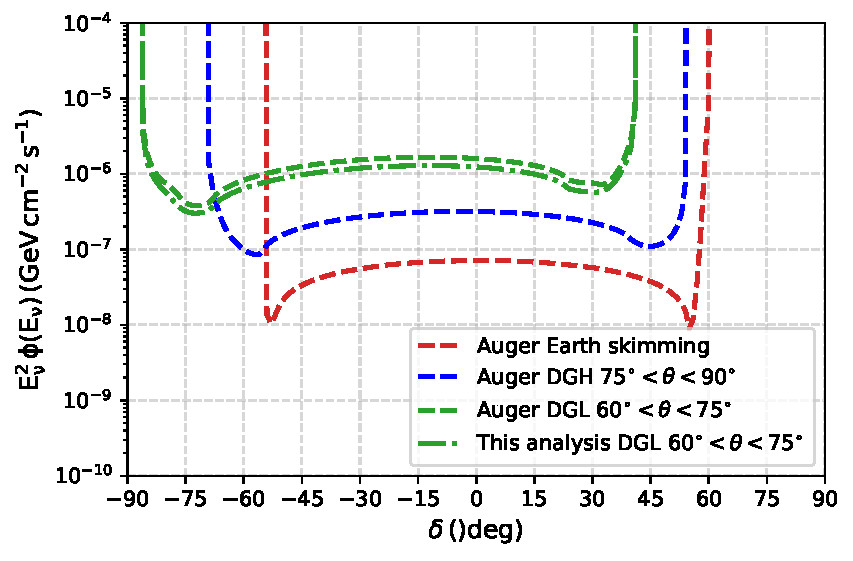
\includegraphics[width=14.5cm]{thesis_figures/PointLimits/Point_comp_combined_3.pdf}
  \caption{Limit comparison 3}
  \label{fig:Dec_limit_comb3}
\end{figure}

\todo{Make table of sources}
The limit obtained in this analysis was then used to constraint some interesting sources which exclusively lie in the DG$_{\text{low}}$ sensitive range. The sources were selected based on their declination and expected neutrino energies which could lie in the region explored.  



%%% Local Variables:
%%% mode: latex
%%% TeX-master: "mythesis"
%%% End:
